\section{Learning the kernel: the Laplace chain}
\label{sec:laplace}

In practice the kernel is unknown and only data are available. This section learns it from noisy sequences, on the
Laplace chain, where the exact score is known and is not linear.

\subsection{Expectation--maximisation through BP}
\label{sec:em}

\begin{figure}[t]
  \centering
  \begin{tikzpicture}[
    box/.style={draw,thick,align=center,font=\small,minimum height=9mm,inner sep=3pt,text width=1.6cm},
    data/.style={box,fill=black!8},
    arr/.style={-{Stealth[length=2mm]},thick},
    lab/.style={font=\small,align=center}]
  \node[font=\small\bfseries,anchor=west] at (-1.1,1.0) {learn};
  \node[data] (d) at (0,0) {noisy\\ sequences};
  \node[box] (p) at (3.1,0) {pair\\ posteriors};
  \node[box] (k) at (6.2,0) {kernel $K_\theta$};
  \draw[arr] (d) -- node[above,lab]{BP} node[below,lab]{E-step} (p);
  \draw[arr] (p) -- node[above,lab]{refit} node[below,lab]{M-step} (k);
  \draw[arr] (k.north) to[out=160,in=20] node[above,lab]{repeat} (d.north);
  \node[font=\small\bfseries,anchor=west] at (-1.1,-1.55) {use};
  \node[data] (x) at (0,-2.5) {noisy\\ sequence $x$};
  \node[box] (m) at (3.1,-2.5) {$\mathbb{E}[a\mid x]$};
  \node[box] (s) at (6.2,-2.5) {score $S_t(x)$};
  \draw[arr] (x) -- node[below,lab]{BP} (m);
  \draw[arr] (m) -- (s);
  \draw[thick,dashed,-{Stealth[length=2mm]}] (k.south) -- (6.2,-1.25) -| (1.55,-2.47);
\end{tikzpicture}

  \caption{Learning and using the kernel. Learn: BP with the current kernel gives the posterior of every pair of
  neighbouring sites (E-step); the kernel is refitted to these pairs (M-step); repeat. Use: BP with the learned
  kernel gives $\E[a\mid x]$, hence the score, at any noise level.}
  \label{fig:em-loop}
\end{figure}

Let $\Kt$ be a parametric family of kernels and $x^{(1)},\dots,x^{(N)}$ noisy training sequences, each at its own
noise level. The likelihood $p_\theta(x)$ sums over all clean sequences compatible with $x$, and BP computes it: it is
the product of the normalisers of the forward messages. Maximising it directly is possible but unnecessary. EM
\cite{dempster1977maximum} splits the problem into the two steps of \cref{fig:em-loop}.

The E-step runs BP with the current parameters $\theta_{\rm old}$ and collects, for every link $k$, the posterior of
the pair,
\begin{align}
  \xi_k(a,a')&=p_{\theta_{\rm old}}(a_k=a,\,a_{k+1}=a'\mid x)\nonumber\\
  &\propto\mu_{\to}^{k}(a)\,K(a'\mid a)\,\ell_t(x_{k+1}\mid a')\,\mu_{\leftarrow}^{k+1}(a').
\end{align}
Summed over links and sequences, $\Xi(a,a')=\sum_{d,k}\xi_k^{(d)}(a,a')$ is the expected number of transitions from
$a$ to $a'$ in the clean data, given what the noisy data show. The M-step then raises
\begin{equation}
  Q(\theta)=\iint\Xi(a,a')\,\log\Kt(a'\mid a)\,\dd a\,\dd a',
  \label{eq:Q}
\end{equation}
the expected log-likelihood of the clean data under the current posterior. With clean data $\Xi$ is the histogram of
observed transitions and the M-step is ordinary maximum likelihood; with noisy data the counts are soft.

The logic is that of following the gradient of an expectation. BP gives the expectation; $\Kt$ is a controlled
function of $\theta$; and the gradient of $Q$ at $\theta_{\rm old}$ is exactly the gradient of the log-likelihood,
$\nabla_\theta\log p_\theta(x)=\nabla_\theta Q(\theta)\rvert_{\theta=\theta_{\rm old}}$ (Fisher's identity,
\cite{louis1982,cappe2005}). Each M-step therefore moves uphill on the likelihood, and the likelihood never decreases
\cite{wu1983}. Two practical consequences follow. First, BP enters the M-step only through $\Xi$, which is fixed
while $\theta$ moves: the gradient of $Q$ goes through $\Kt$ and its normalisation on the grid, never through BP. Any
differentiable family can be trained with ordinary automatic differentiation, a neural network included. Second,
the noise level appears only in the E-step, so the kernel is learned once for all $t$ and no noise schedule is
needed for training.

\subsection{Kernel families}
\label{sec:families}

\begin{figure*}[t]
  \centering
  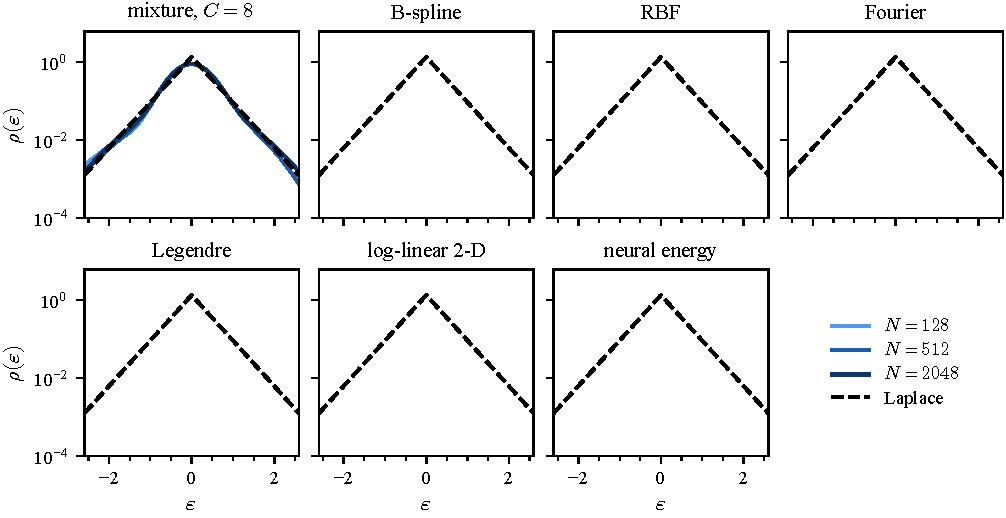
\includegraphics{fig_families}
  \caption{What each kernel family learns. Learned law of the innovation $\varepsilon=a_{k+1}-\alpha a_k$ (for the two
  agnostic families, the learned $K(\varepsilon\mid a=0)$) from $N=128$, $512$ and $2048$ noisy sequences, against the
  Laplace truth (dashed). One seed per $N$. \pending{E56 fits for all panels but the mixture; mixture from exp\_18.}}
  \label{fig:families}
\end{figure*}

\Cref{fig:families} shows what different families learn.
A first choice is a mixture of $C=8$ Gaussians for the innovation,
$\Kt(a'\mid a)=\sum_c\pi_c\Normal(a'-\alpha a;\nu_c,s_c^2)$, with 25 parameters and an almost closed-form M-step. It
learns the coefficient $\alpha$ to within $0.1\%$ from $N=512$ sequences, but it can only approximate the kink by
stacking Gaussians, and the excess kurtosis of its innovation stays $6$ to $25\%$ off (\cref{app:em}).
% src: reports/paper-figures/README.md, fig_em_innovation (exp_18): alpha within 0.1% from N=512 (2.4% at 128); kurtosis 6-25%
Nothing makes a mixture of Gaussians the natural choice. We therefore also expand $\log\Kt$, not $\Kt$, in a basis:
the innovation law is $\phi(\varepsilon)\propto\exp\big(-\lambda\varepsilon^2/2+\sum_mc_m\,b_m(\varepsilon)\big)$ with
$b_m$ cubic B-splines, Gaussian radial basis functions, a truncated Fourier series, or Legendre polynomials, 25
parameters each. Putting the expansion on $\log\Kt$ keeps the kernel positive and makes $Q$ concave in the
coefficients, so every M-step has a unique maximum. Local bases (splines, radial functions) can bend sharply at one
point; global ones (Fourier, Legendre) can only approximate a kink by oscillating.

These are all \emph{shift} families: they assume $a_{k+1}=\alpha a_k+\varepsilon_k$ with $\varepsilon_k$ independent
of $a_k$. Two further families assume nothing. A log-linear kernel expands $\log\Kt(a'\mid a)$ in a tensor B-spline
basis of both arguments (100 parameters). A neural energy kernel sets $\Kt(a'\mid a)\propto\exp(-E_\theta(a,a'))$
with $E_\theta$ a multilayer perceptron with two hidden layers; normalised on the grid, it can represent any smooth
kernel, and it is trained by the same M-step, with a few gradient steps on $Q$ per iteration.
\pending{E56: which family recovers the kink, and at which $N$.}

\subsection{Against neural denoisers}
\label{sec:networks}

\begin{figure}[t]
  \centering
  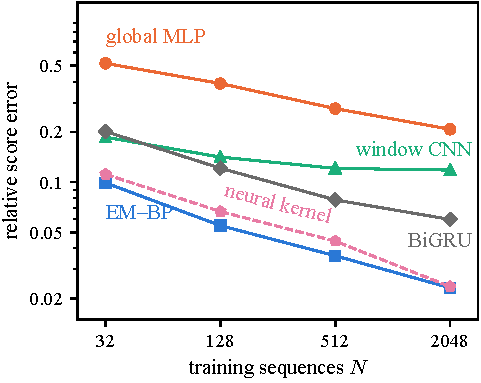
\includegraphics{fig_value_of_structure}
  \caption{Relative score error against the number of training sequences, on the same test sequences. EM--BP with
  the mixture kernel; a global MLP (no locality); a window CNN (locality); BiGRU, the best of six architectures from
  $N=128$ up. Mean over 16 seeds.}
  \label{fig:value-of-structure}
  % src: outputs/E02a/capacity.csv (em_bp, C=8) + outputs/E03/confirm.csv, paired on test bundles (384 of 384 rows)
\end{figure}

\begin{figure}[t]
  \centering
  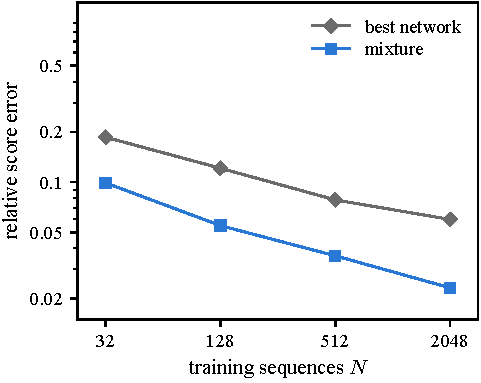
\includegraphics{fig_families_error}
  \caption{Relative score error of every kernel family against $N$, with the best of six networks at each $N$ for
  reference. Same test sequences as \cref{fig:value-of-structure}. \pending{E56.}}
  \label{fig:families-error}
\end{figure}

We compare the learned kernel with neural denoisers trained by denoising score matching \cite{vincent2011connection}:
a global MLP, which has no notion of locality, a window CNN, which has it, and four standard sequence models (BiGRU,
TCN, transformer and U-Net). Each architecture's hyperparameters were screened on separate development seeds and its
checkpoint chosen on a validation set. The networks are trained on the clean training sequences with fresh noise at
every step. EM sees one noisy copy of each sequence, at one noise level, which is a disadvantage for EM.
\note{Appendix D: architectures, parameter counts (MLP 26{,}016, CNN 5{,}505, BiGRU 15{,}169), training recipe.}

\Cref{fig:value-of-structure} puts the three types of model on one plot. With 25 parameters, EM--BP has the lowest
error at every $N$, from $0.099$ at $N=32$ to $0.023$ at $N=2048$.
% src: seed means em_bp 0.0989, 0.0548, 0.0361, 0.0231 (N=32..2048), _paired_e03
The global MLP is $5.8$ to $9.9$ times worse and the window CNN $2.1$ to $5.6$ times worse. The CNN's error barely
improves with $N$ (from $0.14$ at $N=128$ to $0.12$ at $N=2048$), as the window floor of \cref{sec:gaussian}
leads one to expect. The best network at each $N$ is $2.1$ to $2.8$ times worse than EM--BP: the window CNN at $N=32$,
BiGRU above.
% src: mean per-seed ratios, reports/paper-figures/README.md: MLP 5.79/7.95/7.88/9.85, CNN 2.07/2.87/3.45/5.58, BiGRU 2.22/2.45/2.24/2.83
% src: window CNN seed means 0.1861, 0.1413, 0.1209, 0.1181
Both sides here select with the exact score of the validation sequences. Selecting instead by the likelihood of the
noisy validation sequences (EM) and the validation denoising loss (networks) changes the errors by at most $7\%$, and
the kernels stay below the best network in at least 15 of 16 seeds at every $N$ (\cref{app:em}).
% src: tools/core/read_e65.py on outputs/hpc_E65_{k_h0,k_h8,nets} (E65, frozen 4 Nov 2026, 976b595): free/oracle max
% em_bp 1.7%, spline 6.9%, energy 6.9%, networks <= 3.4% (BiGRU); paired below best network 16/16, 16/16, >= 15/16.
% E65's registered P3 is VOID (TCN and transformer missed the 2% reproduction gate): this sentence is descriptive.
\Cref{fig:families-error} adds the other kernel families. \pending{E56: does the neural energy kernel beat the
networks at small $N$, as the registered prediction says.}

\paragraph{The model or the objective?} Trained with the networks' own objective and data, denoising score matching
on the clean sequences with the score computed by a differentiable BP (\cref{app:networks}), the neural energy kernel
is still below the best network in 16 of 16 seeds at every $N$ ($0.018$ against BiGRU's $0.060$ at $N=2048$): the gain
comes from the model. The objective matters too: maximum likelihood on the same sequences is $1.3$ to $2.5$ times more
accurate still.
% src: tools/core/read_e66.py (E66, frozen 4 Nov 2026, 976b595): bp_dsm 0.0557/0.0329/0.0236/0.0183, BiGRU 0.0596 at
% N=2048, P1 16/16 at every N; bp_dsm / E58 energy_h16 (clean ML) = 1.33, 1.31, 1.82, 2.46 at N = 32..2048 (P2 FALSIFIED).

\subsection{Step efficiency}
\label{sec:steps}

\begin{figure*}[t]
  \centering
  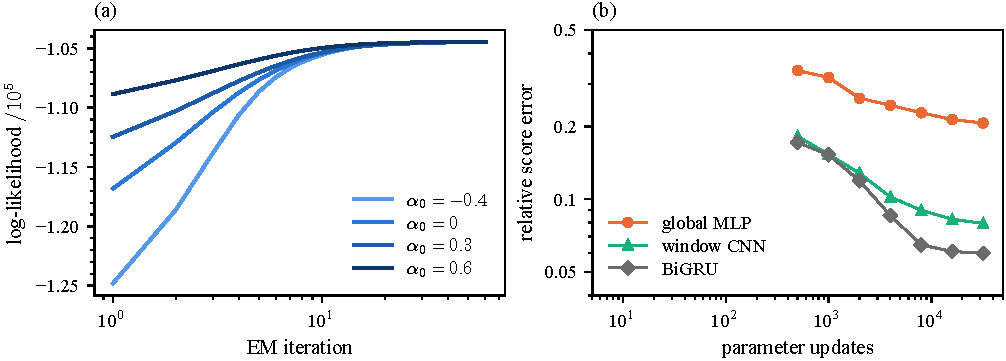
\includegraphics{fig_em_dynamics}
  \caption{Training dynamics. (a) Log-likelihood of the training data against EM iteration, from four starting
  values $\alpha_0$ of the coefficient (mixture kernel, $C=8$). (b) Validation score error against the number of
  parameter updates, $N=2048$: EM iterations for EM--BP, SGD steps for the networks, mean over 16 seeds.
  \pending{E56 EM--BP curve in (b); (a) then from E56, per transition.}}
  \label{fig:em-dynamics}
  % src: (a) Diffusion/research/nongaussian-bp/outputs/frozen/exp_18/em_trace.csv; (b) outputs/E03/confirm.csv val_curve
\end{figure*}

EM needs far fewer parameter updates than gradient training. From every starting point the likelihood rises
monotonically and reaches the same plateau within about twenty iterations (\cref{fig:em-dynamics}a). Parameters that
the likelihood constrains only weakly take longer: over 16 seeds, $\alpha$ settles in a median of 80 updates and the
shape of the innovation law in 229 (at most 638).
% src: memory em-shape-convergence (thesis exp_27, 16 seeds, C=8): rho median 80, shape 229, tail 638
The networks are still improving after $3.2\times10^4$ SGD steps (\cref{fig:em-dynamics}b).

Fewer updates do not mean less time: an EM iteration, a BP pass over all the data, costs 190 to 270 BiGRU steps at
$N=2048$ (\cref{app:compute}). From noisy data the energy kernel reaches the error of BiGRU's selected checkpoint first
in only 7 of 16 seeds at $N=2048$, and its own selected checkpoint later than BiGRU in all 16; from clean data, where an
M-step is one maximum-likelihood fit, it is first in 16 of 16 seeds at every $N\geq128$. At test time BP costs 6 to
20 times a sequence model's forward pass.
% src: tools/core/read_e63.py on outputs/hpc_E63 + E65's curves (E63, frozen 4 Nov 2026, 976b595): s per update at
% N=2048 em_bp 3.40, spline 2.34, energy 2.49, clean_energy 0.482, BiGRU 0.0126 (271x, 187x, 198x); P1 FALSIFIED 7/16,
% P3 16/16, P2 16/16 at N=128/512/2048; use time BP 6972 us vs TCN 1219, transformer 952, U-Net 904, BiGRU 343 us.
% NOTE: the exp_27 figures ("80", "229", "638") come from the memory file, not from a reader script; re-read before submission.

\subsection{Generation}
\label{sec:generation}

With the same ancestral sampler for every model (400 steps down to $t=0.005$; the networks retrained on continuous
levels, \cref{app:generation}), the kernels' samples are closer to the chain. At $N=2048$ the sliced Wasserstein
distance to exact samples is $0.059$ for EM--BP against $0.109$ for BiGRU, the best network, and $0.053$ between two
exact samples. At $N=128$ the clean-data kernel is below every network in at least 7 of 8 seeds, and its residuals'
excess kurtosis is closer to the Laplace value than the best network's in 6 of 8 seeds at both $N$. The samples'
likelihood under the true chain does not rank the models: with the true kernel the sampler scores worse on it than the
window CNN (\cref{app:generation}).
% src: tools/core/read_e64.py on outputs/hpc_E64 (E64, frozen 4 Nov 2026, 976b595), seed means over 8 seeds: SW2 at
% N=2048 em_bp 0.0590, clean_energy 0.0597, bigru_cont 0.1087, exact 0.0532; N=128 clean_energy 0.0966, best net
% window_cont 0.1327; P2 (7/8 at N=128, 8/8 at N=2048), P3 (6/8) CONFIRMED; |loglik gap| oracle_sampler 1.398,
% window_cont 0.373 at N=2048, P4 FALSIFIED.

\subsection{When the data are not Markov}
\label{sec:nonmarkov}

\begin{figure}[t]
  \centering
  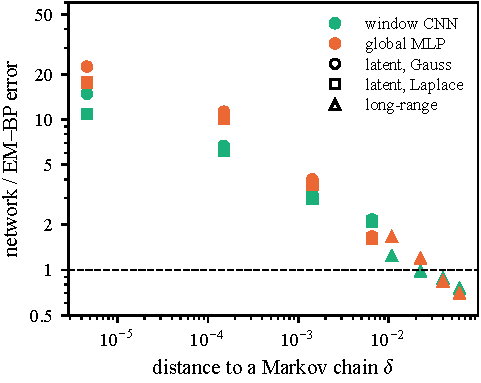
\includegraphics{fig_nonmarkov}
  \caption{Error of a network over that of EM--BP when the data are not Markov, against $\delta$, the distance per
  site from the data to the closest first-order chain. Global latent variable on the Gaussian and the Laplace chain,
  and long-range couplings on the Gaussian chain, each at four strengths. Below the dashed line the network wins.}
  \label{fig:nonmarkov}
  % src: thesis tools/fig_ch10.py::_nonmarkov (frozen exp_21_clean), delta closed form (kl_per_site)
\end{figure}

EM--BP assumes a first-order chain. To see how far this assumption can be wrong, we break it in two ways. A global
latent variable adds one Gaussian draw $g$ per sequence to every site, $a=(y+\beta g)/\sqrt{1+\beta^2}$ with $y$ a
Markov chain; long-range couplings add to the precision of the Gaussian chain a term $\gamma Q_{\rm long}$ that
couples distant sites. Both are measured by the same number, the Kullback--Leibler divergence per site from the
data's covariance to that of the closest first-order chain, $\delta$, in closed form.

\Cref{fig:nonmarkov} shows that both mechanisms, and both chains, fall on one curve. Close to Markov, at
$\delta\approx5\times10^{-6}$, the CNN is $11$ to $15$ times worse than EM--BP and the MLP $18$ to $22$ times.
The advantage shrinks steadily as $\delta$ grows, and the network wins beyond $\delta^\star\approx1$--$2\times10^{-2}$
nats per site for the CNN and $2$--$4\times10^{-2}$ for the MLP.
% src: generator printout: beta=0.1 d=4.61e-6 cnn 14.84/10.92 mlp 22.48/17.64; long-range cnn 1.24 -> 0.97 between d=1.08e-2 and 2.24e-2; mlp 1.19 -> 0.84 between 2.24e-2 and 3.96e-2
Part of the global latent is absorbed into the learned kernel: at $\beta=1$ the learned coefficient moves from $0.848$
to $0.939$, close to that of the best first-order chain.
% src: answers note Q12 (thesis Sec. 8.6, Table 8.9)
\pending{second-order chain $a_k=\phi_1a_{k-1}+\phi_2a_{k-2}+\varepsilon_k$, with EM--BP on the pair state
$(a_{k-1},a_k)$ as the repair.}
